%%%%%%%%%%%%%%%%%%%%%%%%%%%%%%%%%%%%%%%%%%%%%%%%%%%%%%%%%%%%%%%%%%%%%
%% This is a (brief) model paper using the achemso class
%% The document class accepts keyval options, which should include
%% the target journal and optionally the manuscript type. 
%%%%%%%%%%%%%%%%%%%%%%%%%%%%%%%%%%%%%%%%%%%%%%%%%%%%%%%%%%%%%%%%%%%%%
\documentclass[journal=jacsat,manuscript=article]{achemso}

%%%%%%%%%%%%%%%%%%%%%%%%%%%%%%%%%%%%%%%%%%%%%%%%%%%%%%%%%%%%%%%%%%%%%
%% Place any additional packages needed here.  Only include packages
%%, which are essential, to avoid problems later. Do NOT use any
%% packages which require e-TeX (for example etoolbox): the e-TeX
%% extensions are not currently available on the ACS conversion
%% servers.
%%%%%%%%%%%%%%%%%%%%%%%%%%%%%%%%%%%%%%%%%%%%%%%%%%%%%%%%%%%%%%%%%%%%%
% \usepackage[version=3]{mhchem} % Formula subscripts using \ce{}
\usepackage{hyperref}
\usepackage{graphicx}
\graphicspath{ {./resources/} }

%%%%%%%%%%%%%%%%%%%%%%%%%%%%%%%%%%%%%%%%%%%%%%%%%%%%%%%%%%%%%%%%%%%%%
%% If issues arise when submitting your manuscript, you may want to
%% un-comment the next line.  This provides information on the
%% version of every file you have used.
%%%%%%%%%%%%%%%%%%%%%%%%%%%%%%%%%%%%%%%%%%%%%%%%%%%%%%%%%%%%%%%%%%%%%
%%\listfiles

%%%%%%%%%%%%%%%%%%%%%%%%%%%%%%%%%%%%%%%%%%%%%%%%%%%%%%%%%%%%%%%%%%%%%
%% Place any additional macros here.  Please use \newcommand* where
%% possible, and avoid layout-changing macros (which are not used
%% when typesetting).
%%%%%%%%%%%%%%%%%%%%%%%%%%%%%%%%%%%%%%%%%%%%%%%%%%%%%%%%%%%%%%%%%%%%%
\newcommand*\mycommand[1]{\texttt{\emph{#1}}}
\renewcommand{\thefootnote}{\fnsymbol{footnote}}

\author{Vineeth R. Chelur}
\author{U. Deva Priyakumar}
\email{deva@iiit.ac.in}
% \phone{+91 9490441430}
% \author{Yashaswi Pathak}
\affiliation[IIIT-H]
{Center for Computational Natural Sciences \& Bioinformatics, IIIT-H, Hyderabad}

%%%%%%%%%%%%%%%%%%%%%%%%%%%%%%%%%%%%%%%%%%%%%%%%%%%%%%%%%%%%%%%%%%%%%
%% The document title should be given as usual. Some journals require
%% a running title from the author: this should be supplied as an
%% optional argument to \title.
%%%%%%%%%%%%%%%%%%%%%%%%%%%%%%%%%%%%%%%%%%%%%%%%%%%%%%%%%%%%%%%%%%%%%
\title[Predicting the binding-site of a protein for druggable ligands from sequence-based features using Deep Learning]
  {Predicting the binding-site of a protein for druggable ligands from sequence-based features using Deep Learning
%   \footnote{A footnote for the title}
  }

%%%%%%%%%%%%%%%%%%%%%%%%%%%%%%%%%%%%%%%%%%%%%%%%%%%%%%%%%%%%%%%%%%%%%
%% Some journals require a list of abbreviations or keywords to be
%% supplied. These should be set up here, and will be printed after
%% the title and author information, if needed.
%%%%%%%%%%%%%%%%%%%%%%%%%%%%%%%%%%%%%%%%%%%%%%%%%%%%%%%%%%%%%%%%%%%%%
% \abbreviations{IR,NMR,UV}
% \keywords{American Chemical Society, \LaTeX}

%%%%%%%%%%%%%%%%%%%%%%%%%%%%%%%%%%%%%%%%%%%%%%%%%%%%%%%%%%%%%%%%%%%%%
%% The manuscript does not need to include \maketitle, which is
%% executed automatically.
%%%%%%%%%%%%%%%%%%%%%%%%%%%%%%%%%%%%%%%%%%%%%%%%%%%%%%%%%%%%%%%%%%%%%
\begin{document}

%%%%%%%%%%%%%%%%%%%%%%%%%%%%%%%%%%%%%%%%%%%%%%%%%%%%%%%%%%%%%%%%%%%%%
%% The "tocentry" environment can be used to create an entry for the
%% graphical table of contents. It is given here as some journals
%% require that it is printed as part of the abstract page. It will
%% be automatically moved as appropriate.
%%%%%%%%%%%%%%%%%%%%%%%%%%%%%%%%%%%%%%%%%%%%%%%%%%%%%%%%%%%%%%%%%%%%%
% \begin{tocentry}

% Some journals require a graphical entry for the Table of Contents.
% This should be laid out ``print ready'' so that the sizing of the
% text is correct.

% Inside the \texttt{tocentry} environment, the font used is Helvetica
% 8\,pt, as required by \emph{Journal of the American Chemical
% Society}.

% The surrounding frame is 9\,cm by 3.5\,cm, which is the maximum
% permitted for  \emph{Journal of the American Chemical Society}
% graphical table of content entries. The box will not resize if the
% content is too big: instead it will overflow the edge of the box.

% This box and the associated title will always be printed on a
% separate page at the end of the document.

% \end{tocentry}

%%%%%%%%%%%%%%%%%%%%%%%%%%%%%%%%%%%%%%%%%%%%%%%%%%%%%%%%%%%%%%%%%%%%%
%% The abstract environment will automatically gobble the contents
%% if an abstract is not used by the target journal.
%%%%%%%%%%%%%%%%%%%%%%%%%%%%%%%%%%%%%%%%%%%%%%%%%%%%%%%%%%%%%%%%%%%%%
\begin{abstract}
    \noindent\textbf{Motivation}: Protein-drug interactions play important roles in many biological processes. The prediction of the active binding site of a protein helps discover such interactions. The tertiary structure of a protein determines the binding sites available to the drug molecule. But the methods for structure determination are labour-intensive and time-consuming. Hence it becomes important to make predictions using the sequence alone. Deep Learning has been used in a variety of biochemical tasks and has been hugely successful. In this paper, a residual neural network is implemented to predict a protein's most active binding site using features extracted from just the sequence.

    \noindent\textbf{Results}: The model achieves an MCC of 0.53 and an accuracy of 91.2\% on the validation sets averaging across 10-folds. On the test set, an MCC of 0.51 and an accuracy of 90.9\% is obtained.

    \noindent\textbf{Implementation}: \href{https://github.com/crvineeth97/protein-binding-site-prediction}{https://github.com/crvineeth97/protein-binding-site-prediction}
\end{abstract}

%%%%%%%%%%%%%%%%%%%%%%%%%%%%%%%%%%%%%%%%%%%%%%%%%%%%%%%%%%%%%%%%%%%%%
%% Start the main part of the manuscript here.
%%%%%%%%%%%%%%%%%%%%%%%%%%%%%%%%%%%%%%%%%%%%%%%%%%%%%%%%%%%%%%%%%%%%%
\section{Introduction}
\quad The rapid speed of sequencing attained with modern DNA sequencing technology has been instrumental in the sequencing of complete DNA sequences, which leads to faster indirect sequencing of proteins. Although there have been improvements in the determination of the three-dimensional protein structure by techniques such as X-ray crystallography and NMR Spectroscopy, the gap between the number of known sequences (333,201,385 as of July 2020) and the number of known structures (154,706 as of July 2020) is increasing rapidly. Proteins perform a vast array of functions within organisms, and the tertiary structure of a protein can provide important clues about these functions.

Deep Learning is a subfield of machine learning based on artificial neural networks with feature learning. When a deep learning model is fed large amounts of data, it can automatically discover the representations needed for feature detection or classification. Deep learning has been hugely successful in all fields of Natural Sciences, including, but not limited to, binding affinity predictions, protein contact map predictions, and protein-structure predictions. For example, Google's DeepMind team designed a deep learning model, called AlphaFold \cite{senior2020improved}, which represents a considerable advance in protein-structure prediction from a sequence.

In the process of drug design, new medications are found based on the knowledge of a biological target such as a protein. The identification of the potential active binding site of a protein is an essential step in drug design. Predicting the binding site of a protein, based on sequence alone, becomes critical when the three-dimensional structure of the protein is not available.

In this paper, a deep residual neural network is used to make the binary prediction of whether an amino acid residue of the sequence belongs to the primary binding site or not.

\section{Dataset}
\quad For the training and validation of the model, the sc-PDB\cite{desaphy2015sc} dataset (v 2017) is used. The database consists of druggable binding sites of the Protein Data Bank along with prepared protein structures. Thus each sample in the dataset contains the three-dimensional structure of one ligand, one protein, and one site, all stored in mol2 format.

Typically, the complete structure of a protein is unavailable due to missing residues, and hence the full sequence of the protein is obtained from RCSB \cite{burley2019rcsb} website\footnote{Some PDBs in the dataset were obsoleted, and hence the sequences were manually tracked on RCSB, and the corresponding sequences were used. List of obsoleted PDBs is provided in Supporting Information}. A one-to-one mapping of the amino acid in the sequence to the one in the protein mol2 file is required, to know which amino acid belongs to a binding site. This mapping is done by first extracting the protein sequence from the 3D structure. Next, the Needleman-Wunsch dynamic programming algorithm is used to align the sequence extracted from the structure file to the downloaded RCSB sequence. This algorithm is implemented using a modified version of Zhanglab's NW-Align program\cite{NWAlign}. The protein structure file is then reindexed, based on this alignment, to match the indexing of the RCSB sequence. This way, the specific binding residues can be labelled in the RCSB sequence.


The training set consists of 17,594 PDB structures with 28,959 sequences (9519 unique sequences), originating from 1240 organisms, the most abundant being human(28.26\%), (Add the rest here). The dataset was diverse and contained proteins from 1996 different PFAM families (Most abundant needs to be added) and 856 PFAM clans.

This data is split into 10-folds (each containing 1586 structures), based on Uniprot ID, precisely like this paper\cite{stepniewska2020improving}. This split ensures that there is no data leakage between the validation and training set by putting all structures of a single protein in the same fold.

The test set is constructed using all PDBs from 2018 onwards, till 28th February 2020. All PDBs available during this period and having at least one ligand are considered. These are then run through the IChem Toolkit \cite{da2018ichem} to generate a dataset similar to the training set.

The test set consists of 2,274 PDB structures with 3,434 sequences (1889 unique sequences), originating from 548 organisms, the most abundant being human(23.76\%). The test set contained proteins from 882 PFAM families and 452 PFAM clans.

\begin{table}
    \centering
    \begin{tabular}{| p{2.75cm} | p{2.75cm} | p{2.75cm} | p{2.75cm} | p{2.75cm} |}
        \hline
              & $N_{prot}$ & $N_{br}$ & $N_{nbr}$ & $P_{br}(\%)$ \\
        \hline
        Train & 15,860     & 589,329  & 8,725,043 & 6.33         \\
        % Valid & 1586       &          &           &              \\
        Test  & 2,464      & 86,230   & 1,345,646 & 6.02         \\
        \hline
    \end{tabular}
    \caption{Summary of the datasets}
    \label{table:1}
\end{table}

\section{Methods}
\subsection{MSA Generation}
\quad Collections of multiple homologous sequences (called Multiple Sequence Alignments or MSAs) can provide critical information for the modelling of the structure and function of unknown proteins. DeepMSA \cite{zhang2020deepmsa} is an open-source method for sensitive MSA construction, which has homologous sequences and alignments created from multiple sources of databases through complementary hidden Markov model algorithms.

The search is done in 2 stages. In stage 1, the query sequence is searched against the UniClust30 \cite{mirdita2017uniclust} database using HHBlits from HH-suite\cite{remmert2012hhblits} (v2.0.16). If the number of effective sequences is $<$ 128, Stage 2 is performed where the query sequence is searched against the Uniref50 \cite{suzek2015uniref} database using JackHMMER from HMMER \cite{johnson2010hidden} (v3.1b2). Full-length sequences are extracted from the JackHMMER raw hits and converted into a custom HHBlits format database. HHBlits is applied to jump-start the search from Stage 1 sequence MSA against this custom database.


\subsection{Feature Extraction}
\quad There are 9519 unique protein sequences in the sc-PDB dataset and 1889 unique protein sequences in the test set. The MSAs are generated for these sequences using the method described above and stored in PSICOV \cite{jones2012psicov} .aln format. The following features are extracted from the generated MSAs.

\subsubsection{PSSM and IC}
\quad Position Specific Scoring Matrix (PSSM) is a commonly used representation of patterns in biological sequences. PSSMs are derived from MSAs using Easel \cite{potter2018hmmer} and Heinikoff position-based weights so that similar sequences collectively contributed less to PSSM probabilities than diverse sequences.

The information content (IC) of a PSSM gives an idea about how different the PSSM is from a uniform distribution. IC is also derived using Easel.

\subsubsection{Secondary Structure and Solvent Accessibility}
\quad The secondary structure is defined by the pattern of hydrogen bonds formed between the amino hydrogen and carboxyl oxygen atoms in the peptide backbone. It gives an idea of the three-dimensional structure of the protein. The secondary structural elements are alpha helices, beta sheets and turns. PSIPRED (v4.0) \cite{jones1999protein} is used to predict the probability of each state of the 3-state secondary structure for every amino acid in the sequence.

The solvent-accessible surface area is the surface area of a biomolecule that is accessible to a solvent. SOLVPRED from MetaPSICOV 2.0\cite{jones2015metapsicov} is used to predict the relative solvent accessibility (RSA) of every amino acid in the sequence. RSA can be calculated as \\ ${RSA} = {ASA} / {MaxASA}$, where ASA is the solvent-accessible surface area, and MaxASA is the maximum possible solvent accessible surface area for the amino acid residue.

% \subsubsection{SPOT-1D Features}
% \quad As a means to provide better features, SPOT-1D \cite{hanson2019improving} was used to generate the following features: solvent accessibility, half-sphere exposure, contact number, 3-state secondary structure, 8-state secondary structure, and phi, psi, theta and tau torsion angles.

% The first step in the prediction pipeline was to get the ASCII PSSM file in PSI-BLAST format. Then, hhmake was used to generate the HHM file from the MSA. SPIDER3, DCA and CCMPRED predictions were made and stored.

% The second step was to predict the contact map using SPOT-Contact, which used the previous steps predictions.

% Finally, SPOT-1D was used to make the final predictions using all the previous files as input.
% (Need to write in more detail)

\subsection{Deep Learning Model}
\quad Residual neural networks \cite{he2016deep} are immensely popular in image recognition and have been gaining traction in the field of computational Natural Sciences as well. Deep neural networks are difficult to train, but with the introduction of skip connections (shortcuts to jump over some layers) in ResNets, the vanishing gradient problem is avoided. A ResNet consists of multiple basic blocks stacked on top of each other

Have to include the loss function somewhere

Pytorch Lightning Citation - \cite{falcon2019pytorch}

Pytorch Citation\cite{NEURIPS2019_9015}

\vspace{10 mm}
\noindent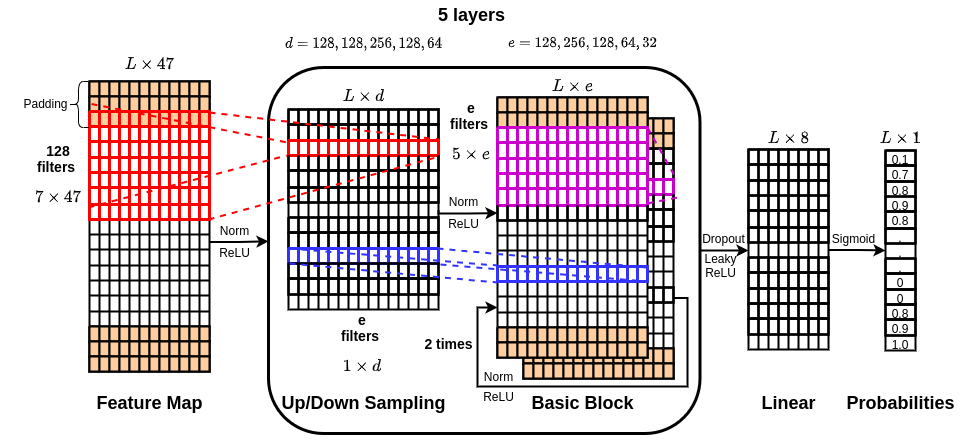
\includegraphics[scale=0.39]{architecture}

\section{Results}
\quad Table of results here

\subsection{Evaluation Metrics}
\subsubsection{Confusion Matrix}
A confusion matrix is a table that allows for the visualization of the performance of a supervised learning algorithm. In the case of binary classification of a residue as a binding residue (BR) or non-binding residue (NBR), the following terminologies can be defined.
\begin{itemize}
    \item True Positive (TP): Number of BRs predicted correctly as BRs.
    \item True Negative (TN): Number of NBRs predicted correctly as NBRs.
    \item False Positive (FP): Number of NBRs predicted incorrectly as BRs.
    \item False Negative (FN): Number of BRs predicted incorrectly as NBRs.
\end{itemize}

\noindent The following metrics can be derived from the confusion matrix

Accuracy: ${ACC} = \frac{TP + TN}{TP + TN + FP + FN}$

Precision: ${PPV} = \frac{TP}{TP + FP}$

Recall: ${TPR} = \frac{TP}{TP + FN}$

F1 score: ${F_1} = \frac{2TP}{2TP + FP + FN}$

Matthews Correlation Coefficient: ${MCC} = \frac{TP \times TN - FP \times FN}{\sqrt{(TP + FP)(TP + FN)(TN + FP)(TN + FN)}}$

(Put all the results in some nice format)

% \subsection{Experiments}
% \quad Should all the things that I tried be included? For eg.

% TAPE Embeddings (Both embeddings) and as a downstream task

% Complementary GAN to try and solve the imbalance

% Using SPOT-1D features

% BiLSTMs, UNet, Transformers

% Window of features using predicted contact maps

% Training on chains separately


\section{Discussion}
\quad

\subsection{Case Studies}
The output from the model of whether a residue belongs to a binding site or not was mapped back to the three-dimensional structure of the protein-ligand complex to get an idea of how well the model is performing. A few of the examples have been chosen to show some perks and flaws of the model
\subsubsection{2X7H}

\subsection{Areas for Improvement}
\quad No good metric to test. As shown in case studies, the model predicts a different binding site.

%%%%%%%%%%%%%%%%%%%%%%%%%%%%%%%%%%%%%%%%%%%%%%%%%%%%%%%%%%%%%%%%%%%%%
%% The "Acknowledgement" section can be given in all manuscript
%% classes.  This should be given within the "acknowledgement"
%% environment, which will make the correct section or running title.
%%%%%%%%%%%%%%%%%%%%%%%%%%%%%%%%%%%%%%%%%%%%%%%%%%%%%%%%%%%%%%%%%%%%%
\begin{acknowledgement}
    The author thanks Yashaswi Pathak for being a fruitful part of the project discussions.

\end{acknowledgement}

%%%%%%%%%%%%%%%%%%%%%%%%%%%%%%%%%%%%%%%%%%%%%%%%%%%%%%%%%%%%%%%%%%%%%
%% The same is true for Supporting information, which should use the
%% suppinfo environment.
%%%%%%%%%%%%%%%%%%%%%%%%%%%%%%%%%%%%%%%%%%%%%%%%%%%%%%%%%%%%%%%%%%%%%
\begin{suppinfo}

    This will usually read something like: ``Experimental procedures and
    characterization data for all new compounds. The class will
    automatically add a sentence pointing to the information on-line:

\end{suppinfo}

%%%%%%%%%%%%%%%%%%%%%%%%%%%%%%%%%%%%%%%%%%%%%%%%%%%%%%%%%%%%%%%%%%%%%
%% The appropriate \bibliography command should be placed here.
%% Notice that the class file automatically sets \bibliographystyle
%% and also names the section correctly.
%%%%%%%%%%%%%%%%%%%%%%%%%%%%%%%%%%%%%%%%%%%%%%%%%%%%%%%%%%%%%%%%%%%%%
\bibliography{achemso-demo}

\end{document}